\documentclass[12pt]{article}
\usepackage[margin=1in]{geometry}
\usepackage{setspace}
\singlespacing % Wacana: single-spaced, 12pt
\usepackage[utf8]{inputenc}
\usepackage[T1]{fontenc}
\usepackage{times}
\usepackage{graphicx}
\usepackage{booktabs}
\usepackage{amsmath}
\usepackage{natbib}
\bibliographystyle{chicago}
\usepackage{hyperref}
\hypersetup{colorlinks=true,linkcolor=blue,citecolor=blue,urlcolor=blue}
\usepackage{caption}
\captionsetup{font=small,labelfont=bf}

\title{What Ancient Texts Remember and Inscriptions Forget:\\
Transformer-Based Evidence for Volcanic Taphonomic Bias\\in Indonesian Textual Records}

\author{Mukhlis Amien\\
\small Lab Data Sains, Universitas Bhinneka Nusantara, Malang, Indonesia\\
\small ORCID: 0000-0002-1848-167X\\
\small \texttt{amien@ubhinus.ac.id}}

\date{}

\begin{document}
\maketitle

\begin{abstract}
Indonesia's indigenous inscriptional record begins around 400 CE, yet external traditions describe Nusantaran societies far earlier. We apply transformer-based NLP to two corpora: 200 passages from twelve external traditions, and 173 Old Javanese, Sanskrit, and Old Malay inscriptions from the DHARMA corpus. Sentence-BERT embeddings show significant \emph{cross-tradition} convergence across all eight concept groups, including a \textsc{volcano} concept spanning all twelve traditions ($z_\mathrm{cross} = 7.1$). In the inscriptions, volcanic-geological themes rank below average in both English and the original Old Javanese, while sacred-mountain discourse ranks highest---an under-representation of the physical mountain. BERTopic detects a (sample-limited) discursive shift around the 929~CE Mataram transition (Fisher's exact $p = 0.0003$, $n = 46$). Indonesia's textual record is shaped not only by physical survival but by genre selection---taphonomic bias at the level of discourse, not stratigraphy.
\end{abstract}

\noindent\textbf{Keywords:} computational textual archaeology, Sentence-BERT, BERTopic, Old Javanese epigraphy, Nusantara, volcanic taphonomy, DHARMA inscriptions, semantic convergence

\section{Introduction}

Indonesia presents one of the sharpest paradoxes in global archaeology.
The archipelago was home to \textit{Homo erectus} for over a million years, lies at the crossroads of two major maritime trade routes, and is referenced in Greek, Roman, Indian, Chinese, Arab, and Persian sources from the 3rd century BCE onward.
Yet the indigenous inscriptional record begins only around 400 CE, and the number of known archaeological sites in Java's volcanic zones is a fraction of what comparable regions in Japan, Italy, or Mesoamerica have produced.

The VOLCARCH framework \citep[submitted]{Amien2026a} proposes that this ``archaeological darkness'' results from three interlocking taphonomic biases: (1) volcanic burial, which progressively conceals sites at rates of 2.4--6.2 mm/year; (2) institutional survey deficit, with Indonesia conducting roughly 100--200 times fewer rescue excavations per unit area than Japan \citep[submitted]{Amien2026a}; and (3) textual genre taphonomy---the possibility that the types of text preserved in stone systematically exclude certain kinds of information.

This paper addresses the third bias computationally.
We ask: do independent external textual traditions preserve evidence of Nusantaran societies where the indigenous archaeological and inscriptional record is sparse?
And if so, what does the indigenous inscriptional record choose to remember---and what does it forget?

To answer these questions, we deploy three transformer-based NLP methods on two distinct corpora.
The first corpus comprises 200 translated passages from 12 ancient traditions spanning 3,065 years (1700 BCE--1365 CE), ranging from Mesopotamian clove finds to Ming dynasty maritime accounts.
The second is the DHARMA EpiDoc corpus of 268 Old Javanese, Sanskrit, and Old Malay inscriptions digitized by the DHARMA project \citep{DHARMA2024}.
By embedding both corpora in the same semantic space, we can measure what external traditions converge on and what inscriptions systematically exclude.

\subsection{Research questions}

\begin{enumerate}
    \item Do 12 independent textual traditions converge semantically on Nusantaran themes, or is the convergence an artefact of shared sources?
    \item What latent topics emerge when BERTopic is applied to a cross-tradition corpus about Nusantara?
    \item How does inscriptional discourse relate to physical landscape---specifically, do inscriptions encode volcanic or geological features?
    \item Does the 929 CE political collapse (Mataram) mark a detectable discursive discontinuity in the epigraphic record?
\end{enumerate}

These questions are novel in two respects.
No prior study has applied Sentence-BERT or BERTopic to Old Javanese epigraphy, and no study has tested cross-tradition semantic convergence across 12 independent traditions simultaneously.
The closest precedents are neural NER on Sumerian cuneiform \citep{PagePerron2017}, the Ithaca system for restoring and dating Greek inscriptions \citep{Assael2022}, and topic modelling on Early Modern English texts \citep{Manjavacas2019}.
Our work extends the computational epigraphy paradigm to Southeast Asia and, uniquely, combines it with a cross-cultural convergence methodology.

\subsection{Why this matters}

If the textual record is taphonomically biased---if inscriptions systematically exclude physical geography while external sources systematically include it---then the absence of volcanic references in Indonesian epigraphy is not evidence that ancient Javanese were unaware of volcanism.
It is evidence that the inscriptional genre was designed for a different purpose: legitimating royal authority and recording administrative transactions, not describing the physical world.
This distinction has implications for how we use inscriptions as archaeological proxies, and more broadly for how we interpret silence in the historical record.

% (conceptual framework slide removed for journal submission; the three biases are described in the text)


\section{Background}

\subsection{The archaeological darkness problem}

The concept of ``archaeological darkness'' describes periods or regions where the material record is disproportionately sparse relative to what external evidence suggests should exist.
In Indonesia, the darkness is extreme: the archipelago was home to \textit{Homo erectus} for over a million years, lies at the intersection of the Indian Ocean and Pacific trade networks, and was the source of spices valued by Mediterranean civilizations from at least 1700 BCE---yet the indigenous inscriptional record begins only around 400 CE \citep{Coedes1968, Vogel1918}.

The standard interpretation treats this gap as evidence of absence: complex Nusantaran societies simply did not exist before they produced inscriptions.
An alternative interpretation is that the gap reflects \emph{taphonomic bias}---the systematic destruction or concealment of evidence through geological, institutional, and textual processes \citep{Schiffer1987}.
The VOLCARCH framework \citep[submitted]{Amien2026a} identifies three interlocking mechanisms: volcanic burial at 2.4--6.2~mm/year that physically conceals sites \citep{Lavigne2000}; institutional survey deficit, with Indonesia conducting 100--200 times fewer rescue excavations per unit area than comparably volcanic Japan; and textual genre taphonomy, the possibility that inscriptional genres systematically exclude certain categories of information.
This paper addresses the third mechanism computationally.

\subsection{Textual sources for pre-modern Nusantara}

References to the Indonesian archipelago appear in at least 12 distinct textual and material traditions.
The earliest is archaeochemical: clove residues in a vessel from Terqa, Syria, dated to approximately 1700 BCE \citep{Rageot2023}, implying a trade network connecting eastern Indonesia to the Near East over three millennia before the first Nusantaran inscription.
The Jataka Tales (\textit{c.} 4th--3rd century BCE) reference Suvarnabhumi, an Indianized toponym for the ``Golden Land'' widely identified with insular Southeast Asia.
Greek geographers including Eratosthenes (\textit{c.} 235 BCE) and Ptolemy (150 CE) mention Chryse and Iabadiu, while Roman encyclopaedists (Pliny, Pomponius Mela) describe Nusantaran spices.
Chinese dynastic histories from the 3rd century CE onward provide increasingly detailed accounts of Javanese kingdoms, and Arab geographers from the 9th century offer independent descriptions.
Persian cosmographies, Tamil Sangam literature, Indian Buddhist pilgrim accounts, and archaeological chemistry (camphor, cinnamon, benzoin residues) complete the picture.

These traditions differ in language, genre, purpose, and geographic perspective.
Their convergence on insular Southeast Asia as a source of spices, gold, camphor, and complex polities constitutes a form of independent corroboration that is particularly valuable where indigenous records are sparse.
The question is whether this convergence is recoverable computationally---whether transformer-based NLP can detect the shared semantic signal beneath the surface diversity of 12 traditions spanning 3,065 years.

\subsection{NLP in archaeology and epigraphy}

The application of transformer-based NLP to ancient texts is a growing field within digital humanities, though applications to Southeast Asian material remain virtually absent.
Three lines of prior work are directly relevant.

\textbf{Named entity recognition on ancient administrative texts.}
\citet{PagePerron2017} pioneered NER on Sumerian administrative cuneiform tablets from the Ur III period, demonstrating that neural sequence labelling could extract personal names, commodities, and quantities from highly formulaic but fragmentary texts.
Their work showed that even with small training sets, modern NLP architectures could outperform rule-based systems on ancient administrative corpora.

\textbf{Deep learning for inscription restoration and dating.}
\citet{Assael2022} developed Ithaca, a transformer-based system published in \textit{Nature} that restores damaged text, dates, and geographically attributes ancient Greek inscriptions with accuracy competitive with expert epigraphers.
Ithaca was trained on 78,608 inscriptions from the Packard Humanities Institute corpus and demonstrated that dense neural representations could capture both linguistic and historical patterns in inscriptional data.

\textbf{Semantic embeddings for historical text analysis.}
\citet{Manjavacas2019} applied contextual embeddings to Early Modern texts, showing that semantic similarity metrics could capture thematic relationships invisible to bag-of-words methods.
Dense sentence embeddings---particularly Sentence-BERT \citep{Reimers2019}---have subsequently been applied to various historical corpora, enabling semantic search, clustering, and cross-document comparison without task-specific fine-tuning.

Topic modelling has been applied to historical corpora ranging from 18th-century newspapers \citep{Blei2003} to medieval charters, but to our knowledge, no study has applied BERTopic \citep{Grootendorst2022}---which combines SBERT embeddings with HDBSCAN clustering and class-based TF-IDF---to ancient inscriptions of any tradition.

In Southeast Asian studies, computational approaches to inscriptions remain rare.
The DHARMA project \citep{DHARMA2024} has digitized hundreds of inscriptions in TEI-XML format, creating an unprecedented machine-readable corpus of Old Javanese, Sanskrit, Old Malay, and Old Sundanese texts.
However, computational analysis beyond keyword concordances and palaeographic classification has not been published.
This paper represents the first transformer-based NLP applied to Old Javanese epigraphy, and the first cross-tradition semantic convergence test spanning 12 ancient traditions simultaneously.

\subsection{The 929 CE divide}

The year 929 CE marks the end of the Mataram kingdom in Central Java and the beginning of East Javanese political ascendancy.
The causes are debated: a catastrophic Merapi eruption, political fragmentation, or voluntary relocation have all been proposed \citep{Degroot2009}.
Whatever the cause, the inscriptional record shifts geographically and, as we will show, discursively.
The 929 CE divide provides a natural experiment for testing whether political disruption produces detectable changes in what inscriptions encode.


\section{Data}

\subsection{Corpus 1: Cross-tradition Nusantara references}

We compiled a corpus of 200 translated passages from 12 textual traditions referencing Nusantara (Table~\ref{tab:corpus1}).
Each entry includes an English translation of the relevant passage, the tradition of origin, approximate date, and thematic tags.
Passages were selected based on a single criterion: they must contain a direct reference to Nusantaran geography, commodities, peoples, or polities.

\begin{table}[htbp]
\centering
\caption{Cross-tradition corpus composition (E089 v5).}
\label{tab:corpus1}
\begin{tabular}{lrl}
\toprule
\textbf{Tradition} & \textbf{N} & \textbf{Date range} \\
\midrule
Chinese     & 42 & 130--1433 CE \\
Arab        & 25 & 851--1400 CE \\
Nusantaran  & 22 & 400--1365 CE \\
Chemical    & 19 & 1700 BCE--1200 CE \\
European    & 16 & 1292--1515 CE \\
Linguistic  & 12 & 2000 BCE--1400 CE \\
Indian (Sanskrit) & 12 & 350 BCE--600 CE \\
Tamil       & 12 & 200 BCE--600 CE \\
Indian (Pali)     & 11 & 350--500 BCE \\
Greek       & 11 & 235 BCE--550 CE \\
Roman       & 11 & 43--166 CE \\
Persian     &  7 & 982--1340 CE \\
\midrule
\textbf{Total} & \textbf{200} & \textbf{1700 BCE--1515 CE} \\
\bottomrule
\end{tabular}
\end{table}

The corpus was constructed through systematic mining of published translations, augmented by AI-assisted extraction.
The 12 traditions include two that are non-textual: \textit{Chemical} (archaeometric analyses of traded commodities such as cloves, camphor, and cinnamon) and \textit{Linguistic} (reconstructed Proto-Austronesian and Proto-Malayo-Polynesian terms for geographic and material concepts).

\subsection{Corpus 2: DHARMA inscriptions}

The second corpus comprises 268 inscriptions from the DHARMA EpiDoc project, encoded in TEI-XML.
Of these, 173 have English translations and were used for semantic embedding; 46 are both dated and translated, and were used for diachronic topic modelling.
Languages represented include Old Javanese (\textit{kaw-Latn}, $n = 89$), Sanskrit (\textit{san-Latn}, $n = 59$), Old Sundanese (\textit{osn-Latn}, $n = 14$), and Old Malay (\textit{omy-Latn}, $n = 10$).
The dated subset spans the 8th through 14th centuries CE, with the densest coverage in C9 ($n = 17$) and C10 ($n = 12$).


\section{Methods}

The computational pipeline proceeds in four stages: encoding ancient texts as dense vectors with Sentence-BERT (384 dimensions), reducing dimensionality with UMAP for visualization, discovering latent topics with BERTopic, and testing semantic convergence by Monte Carlo. The pipeline is fully reproducible and requires no training data.

\subsection{Sentence-BERT encoding}

All passages from both corpora were encoded using Sentence-BERT (all-MiniLM-L6-v2; \citealp{Reimers2019}) on a CUDA-enabled GPU (NVIDIA RTX 4080).
This model maps text to a 384-dimensional dense vector space in which cosine similarity reflects semantic relatedness.
Although trained on modern English, prior work has shown that SBERT embeddings capture thematic similarity in historical and translated texts \citep{Manjavacas2019}.
The embedding step is deterministic and produces a matrix of $N \times 384$ for each corpus.

\subsection{Cross-tradition semantic convergence}

For the cross-tradition corpus (200 passages), we defined eight concept groups: \textsc{java}, \textsc{sumatra\_gold}, \textsc{camphor\_barus}, \textsc{spice\_trade}, \textsc{maritime\_voyage}, \textsc{volcano}, \textsc{buddhist\_world}, and \textsc{metal\_trade}.
Each group was populated by tagging passages whose content relates to the concept, regardless of tradition.

To test whether passages \emph{from different traditions} converge---rather than merely measuring within-group topical coherence---we use a tradition-controlled statistic. For each group we compute $S_\mathrm{cross}$, the mean cosine similarity of pairs whose two passages come from \emph{different} traditions, and compare it to a null distribution of random cross-tradition pairs drawn from the full corpus (5{,}000 bootstrap resamples).
The resulting $z$-scores and $p$-values are Benjamini--Hochberg corrected across the eight groups; we also report $S_\mathrm{within}$ (same-tradition pairs) for comparison.
This isolates genuine cross-tradition agreement from within-tradition stylistic homogeneity and avoids parametric assumptions about the embedding distribution.

\subsection{UMAP clustering and BERTopic}

Dimensionality reduction was performed using UMAP \citep{McInnes2018} ($n\_components = 2$, $n\_neighbors = 15$, $min\_dist = 0.1$) followed by HDBSCAN clustering \citep{McInnes2017} ($min\_cluster\_size = 4$).
Clusters were evaluated for cross-tradition composition: a cluster containing passages from multiple traditions is ``content-driven'' (grouped by topic), while a tradition-pure cluster is ``culture-driven'' (grouped by literary genre or perspective).

BERTopic \citep{Grootendorst2022} was applied to the 200-passage corpus to discover latent topics without supervision.
BERTopic combines SBERT embeddings with UMAP dimensionality reduction, HDBSCAN clustering, and class-based TF-IDF to extract interpretable topic labels.

\subsection{Epigraphic semantic search}

For the DHARMA corpus (173 translated inscriptions), we defined seven thematic queries:
\begin{enumerate}
    \item village administration and land grants
    \item mountain worship and sacred peaks
    \item water infrastructure, irrigation, dams
    \item royal genealogy and succession
    \item tax collection and economic regulation
    \item Buddhist monastery and religious donation
    \item volcanic landscape, fire mountain
\end{enumerate}

Each query was embedded using the same SBERT model, and the top-10 nearest inscriptions were retrieved by cosine similarity.
Mean similarity per query measures how close each theme is to the overall inscriptional discourse.

\subsection{Temporal centroid drift}

For dated inscriptions, we computed a centroid embedding per century and measured pairwise cosine distances between consecutive centuries.
This produces a ``semantic drift'' profile showing which century transitions involved the largest discursive changes.
The pre-929 versus post-929 CE centroid distance was also computed.

\subsection{Diachronic BERTopic}

BERTopic was applied separately to the 46 dated inscriptions.
Topics were cross-tabulated against century and against the pre-929/post-929 divide.
Statistical significance was assessed using a chi-square test on the topic $\times$ period contingency table and Fisher's exact tests for individual topics.

\subsection{Cross-lingual validation}

A key limitation of the above pipeline is its reliance on English translations.
To assess whether the semantic patterns observed in translation are artefacts of the translation process, we conducted a cross-lingual validation using two multilingual transformer models on the original Old Javanese, Sanskrit, and Old Malay texts:

\begin{enumerate}
    \item \textbf{XLM-RoBERTa-base} \citep{Conneau2020}: a 100-language token-level model with mean pooling, applied to 207 inscriptions with original text ($>$50 characters).
    \item \textbf{Multilingual SBERT} (paraphrase-multilingual-MiniLM-L12-v2): a sentence-level multilingual model trained on parallel corpora in 50+ languages.
\end{enumerate}

For the 112 inscriptions with both original text and English translation, we computed pairwise similarity matrices in both original-language and English embedding spaces, then measured Spearman rank correlation between the two similarity structures.
A significant positive correlation indicates that the English-only analysis captures real semantic structure present in the original texts.
The same seven thematic queries were executed against original-language embeddings for direct comparison.


\section{Results}

\subsection{Cross-tradition semantic convergence}

A naive within-group similarity test (intra-group mean vs.\ random pairs) cannot distinguish genuine cross-tradition convergence from within-tradition homogeneity: a group dominated by one tradition would score highly for either reason. We therefore use a \emph{tradition-controlled} test. For each concept group we compute the mean cosine similarity of pairs drawn from \emph{different} traditions ($S_\mathrm{cross}$) and compare it to a null of random cross-tradition pairs from the full corpus (mean $0.305$; 5{,}000 bootstrap resamples; Benjamini--Hochberg corrected across the eight groups).

All eight groups show significant cross-tradition convergence (Table~\ref{tab:convergence}): $S_\mathrm{cross}$ exceeds the random cross-tradition baseline in every case, with $z$ from $3.6$ (\textsc{metal\_trade}) to $32.2$ (\textsc{spice\_trade}). The \textsc{volcano} concept achieves $z = 7.1$ across 12 traditions, with no single tradition contributing more than 19\% of its passages---so volcanic awareness is a genuinely pan-tradition theme, not within-tradition homogeneity. Within-tradition pairs are, as expected, somewhat more similar than cross-tradition pairs ($S_\mathrm{within} = 0.39$--$0.49$ vs.\ $S_\mathrm{cross} = 0.31$--$0.39$), but the cross-tradition signal remains well above chance for every group, indicating convergence \emph{across} independent traditions rather than mere stylistic homogeneity within them.

\begin{table}[htbp]
\centering
\caption{Cross-tradition semantic convergence (tradition-controlled). For each concept group: number of passages ($N$), number of traditions, mean within-tradition ($S_\mathrm{within}$) and cross-tradition ($S_\mathrm{cross}$) pairwise cosine similarity, and the $z$-score of $S_\mathrm{cross}$ against a random cross-tradition baseline (mean $0.305$; 5{,}000 bootstrap, Benjamini--Hochberg corrected). All eight groups converge \emph{across} traditions.}
\label{tab:convergence}
\begin{tabular}{lrrrrr}
\toprule
\textbf{Concept group} & \textbf{N} & \textbf{Trad.} & \textbf{$S_\mathrm{within}$} & \textbf{$S_\mathrm{cross}$} & \textbf{$z_\mathrm{cross}$} \\
\midrule
\textsc{spice\_trade}      & 76  & 10 & 0.477 & 0.373 & 32.2 \\
\textsc{camphor\_barus}    & 51  & 10 & 0.494 & 0.389 & 25.4 \\
\textsc{sumatra\_gold}     & 75  & 11 & 0.474 & 0.356 & 24.1 \\
\textsc{maritime\_voyage}  & 128 & 12 & 0.405 & 0.328 & 18.9 \\
\textsc{java}              & 82  & 11 & 0.464 & 0.338 & 16.5 \\
\textsc{volcano}           & 54  & 12 & 0.422 & 0.326 &  7.1 \\
\textsc{buddhist\_world}   & 23  &  8 & 0.444 & 0.331 &  3.6 \\
\textsc{metal\_trade}      & 135 & 12 & 0.389 & 0.309 &  3.6 \\
\bottomrule
\end{tabular}
\\[2pt]
{\footnotesize All $z_\mathrm{cross} > 1.96$; all $p < 0.001$ (BH-corrected). Dominant-tradition share 0.17--0.27, i.e.\ no group is driven by a single tradition.}
\end{table}

Notably, \textsc{java} converges across traditions ($z_\mathrm{cross} = 16.5$) despite the heterogeneity of passages about Java---ranging from Ptolemy's geographic coordinates to Faxian's Buddhist pilgrimage to Song dynasty diplomatic records.
The SBERT embeddings capture a shared semantic core beneath the surface-level diversity.

\begin{figure}[htbp]
\centering
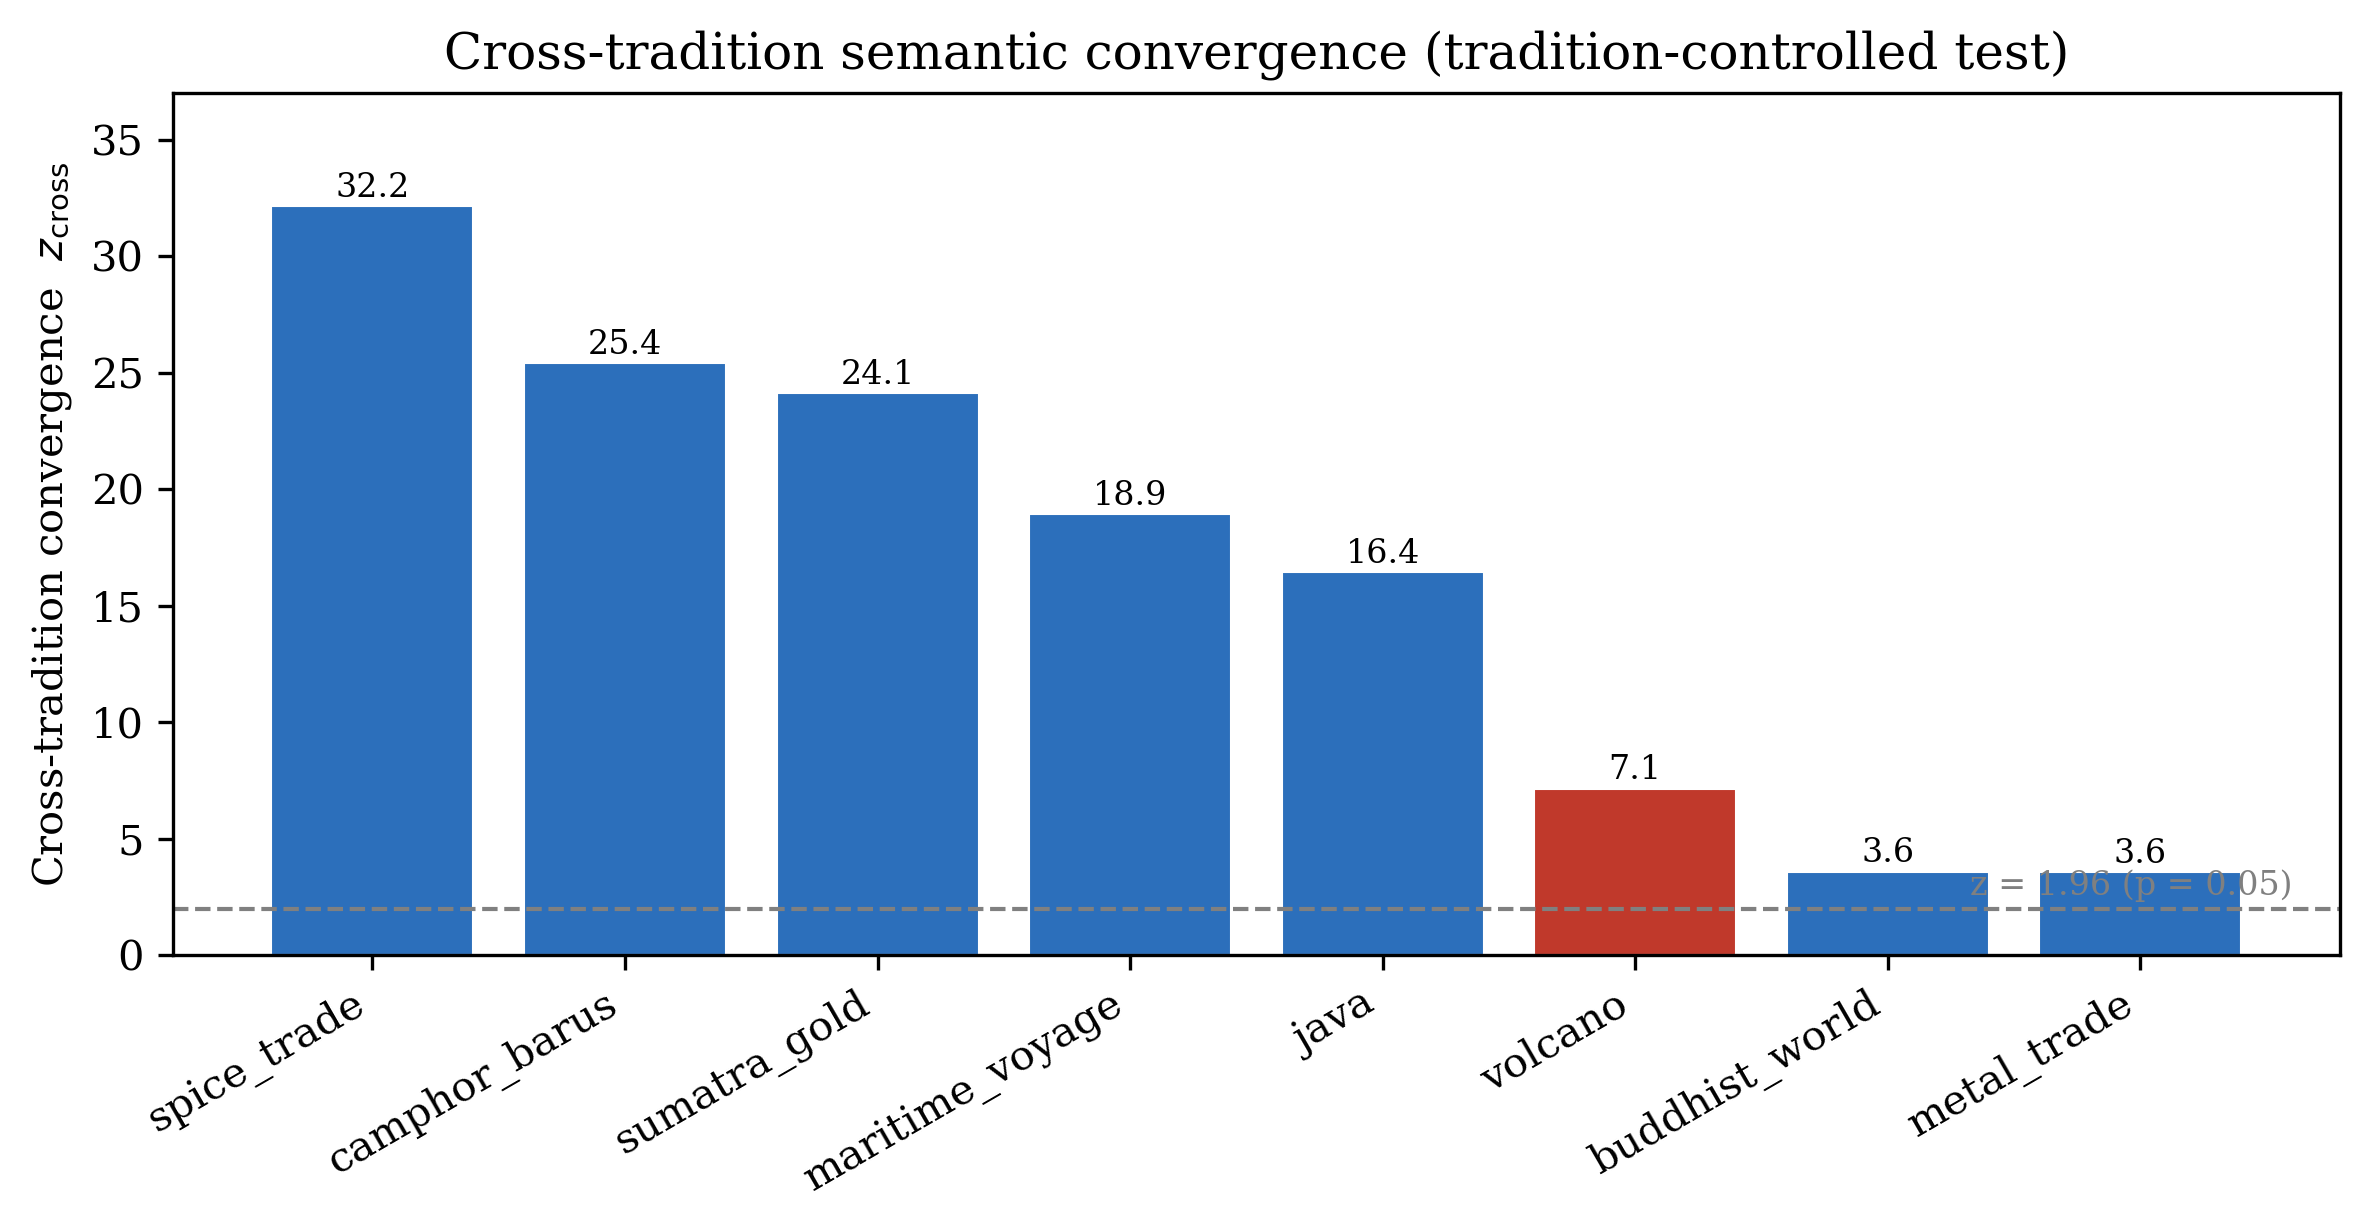
\includegraphics[width=\textwidth]{figures/fig3_convergence_zscores.png}
\caption{Cross-tradition convergence $z$-scores for eight concept groups (tradition-controlled test: $S_\mathrm{cross}$ vs.\ a random cross-tradition baseline). All eight groups exceed the significance threshold ($z > 1.96$, Benjamini--Hochberg corrected).}
\label{fig:convergence}
\end{figure}

\subsection{Latent topics in the cross-tradition corpus}

BERTopic discovers 16 topics (Figure~\ref{fig:umap}).
Several are directly relevant to the VOLCARCH framework:
\begin{itemize}
    \item \textbf{Topic 4} (14 documents): ``volcanic, Sanskrit, inscriptions, Javanese, Malay''---a volcanic-linguistic nexus linking volcanic awareness to epigraphic sources
    \item \textbf{Topic 12} (5 documents): ``mountain, slopes, clouds, temples, smoke''---volcanic landscape as described in literary and travel sources
    \item \textbf{Topic 0} (25 documents): ``ship, sea, merchant, gold''---maritime trade, the dominant discourse across all traditions
    \item \textbf{Topic 8} (7 documents): ``inscription, Saka, royal, Suvarnadvipa, king''---Nusantaran epigraphy as its own thematic cluster
\end{itemize}

UMAP clustering reveals that 57\% of HDBSCAN clusters (12/21) are cross-tradition, confirming that passages cluster by \emph{content} rather than by cultural origin (Figure~\ref{fig:umap}).

\begin{figure}[htbp]
\centering
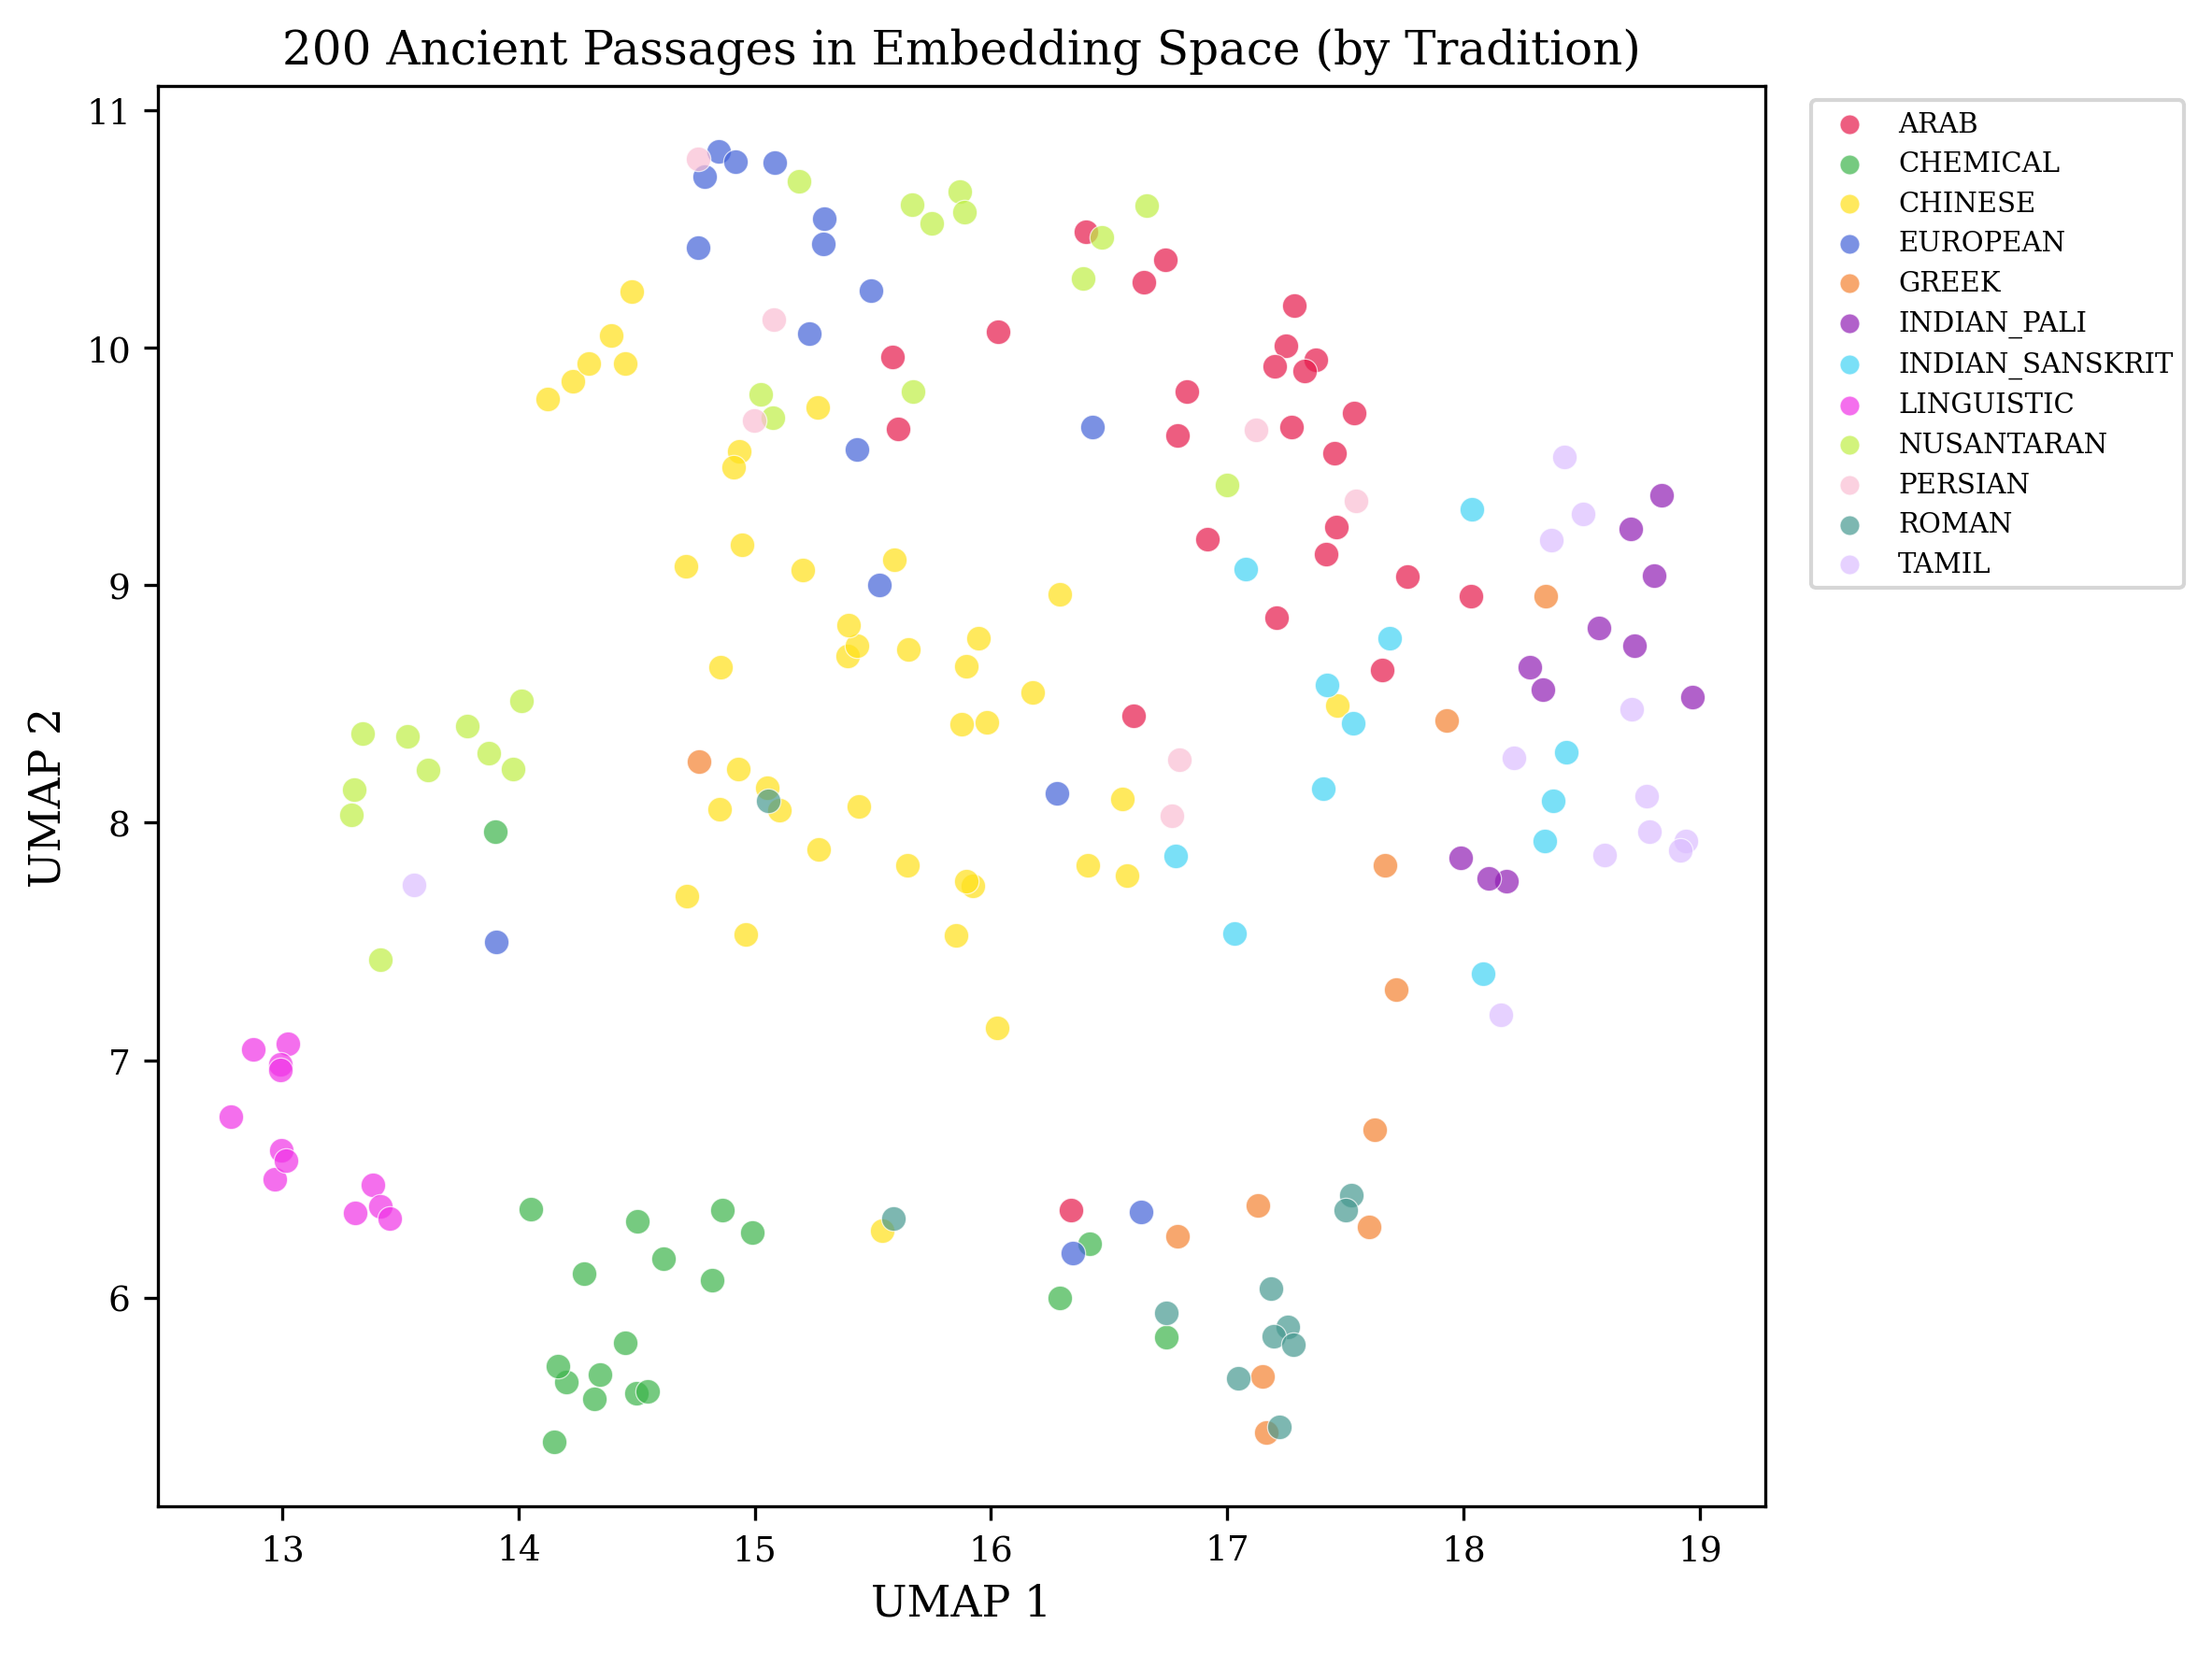
\includegraphics[width=0.48\textwidth]{figures/fig1_umap_tradition.png}
\hfill
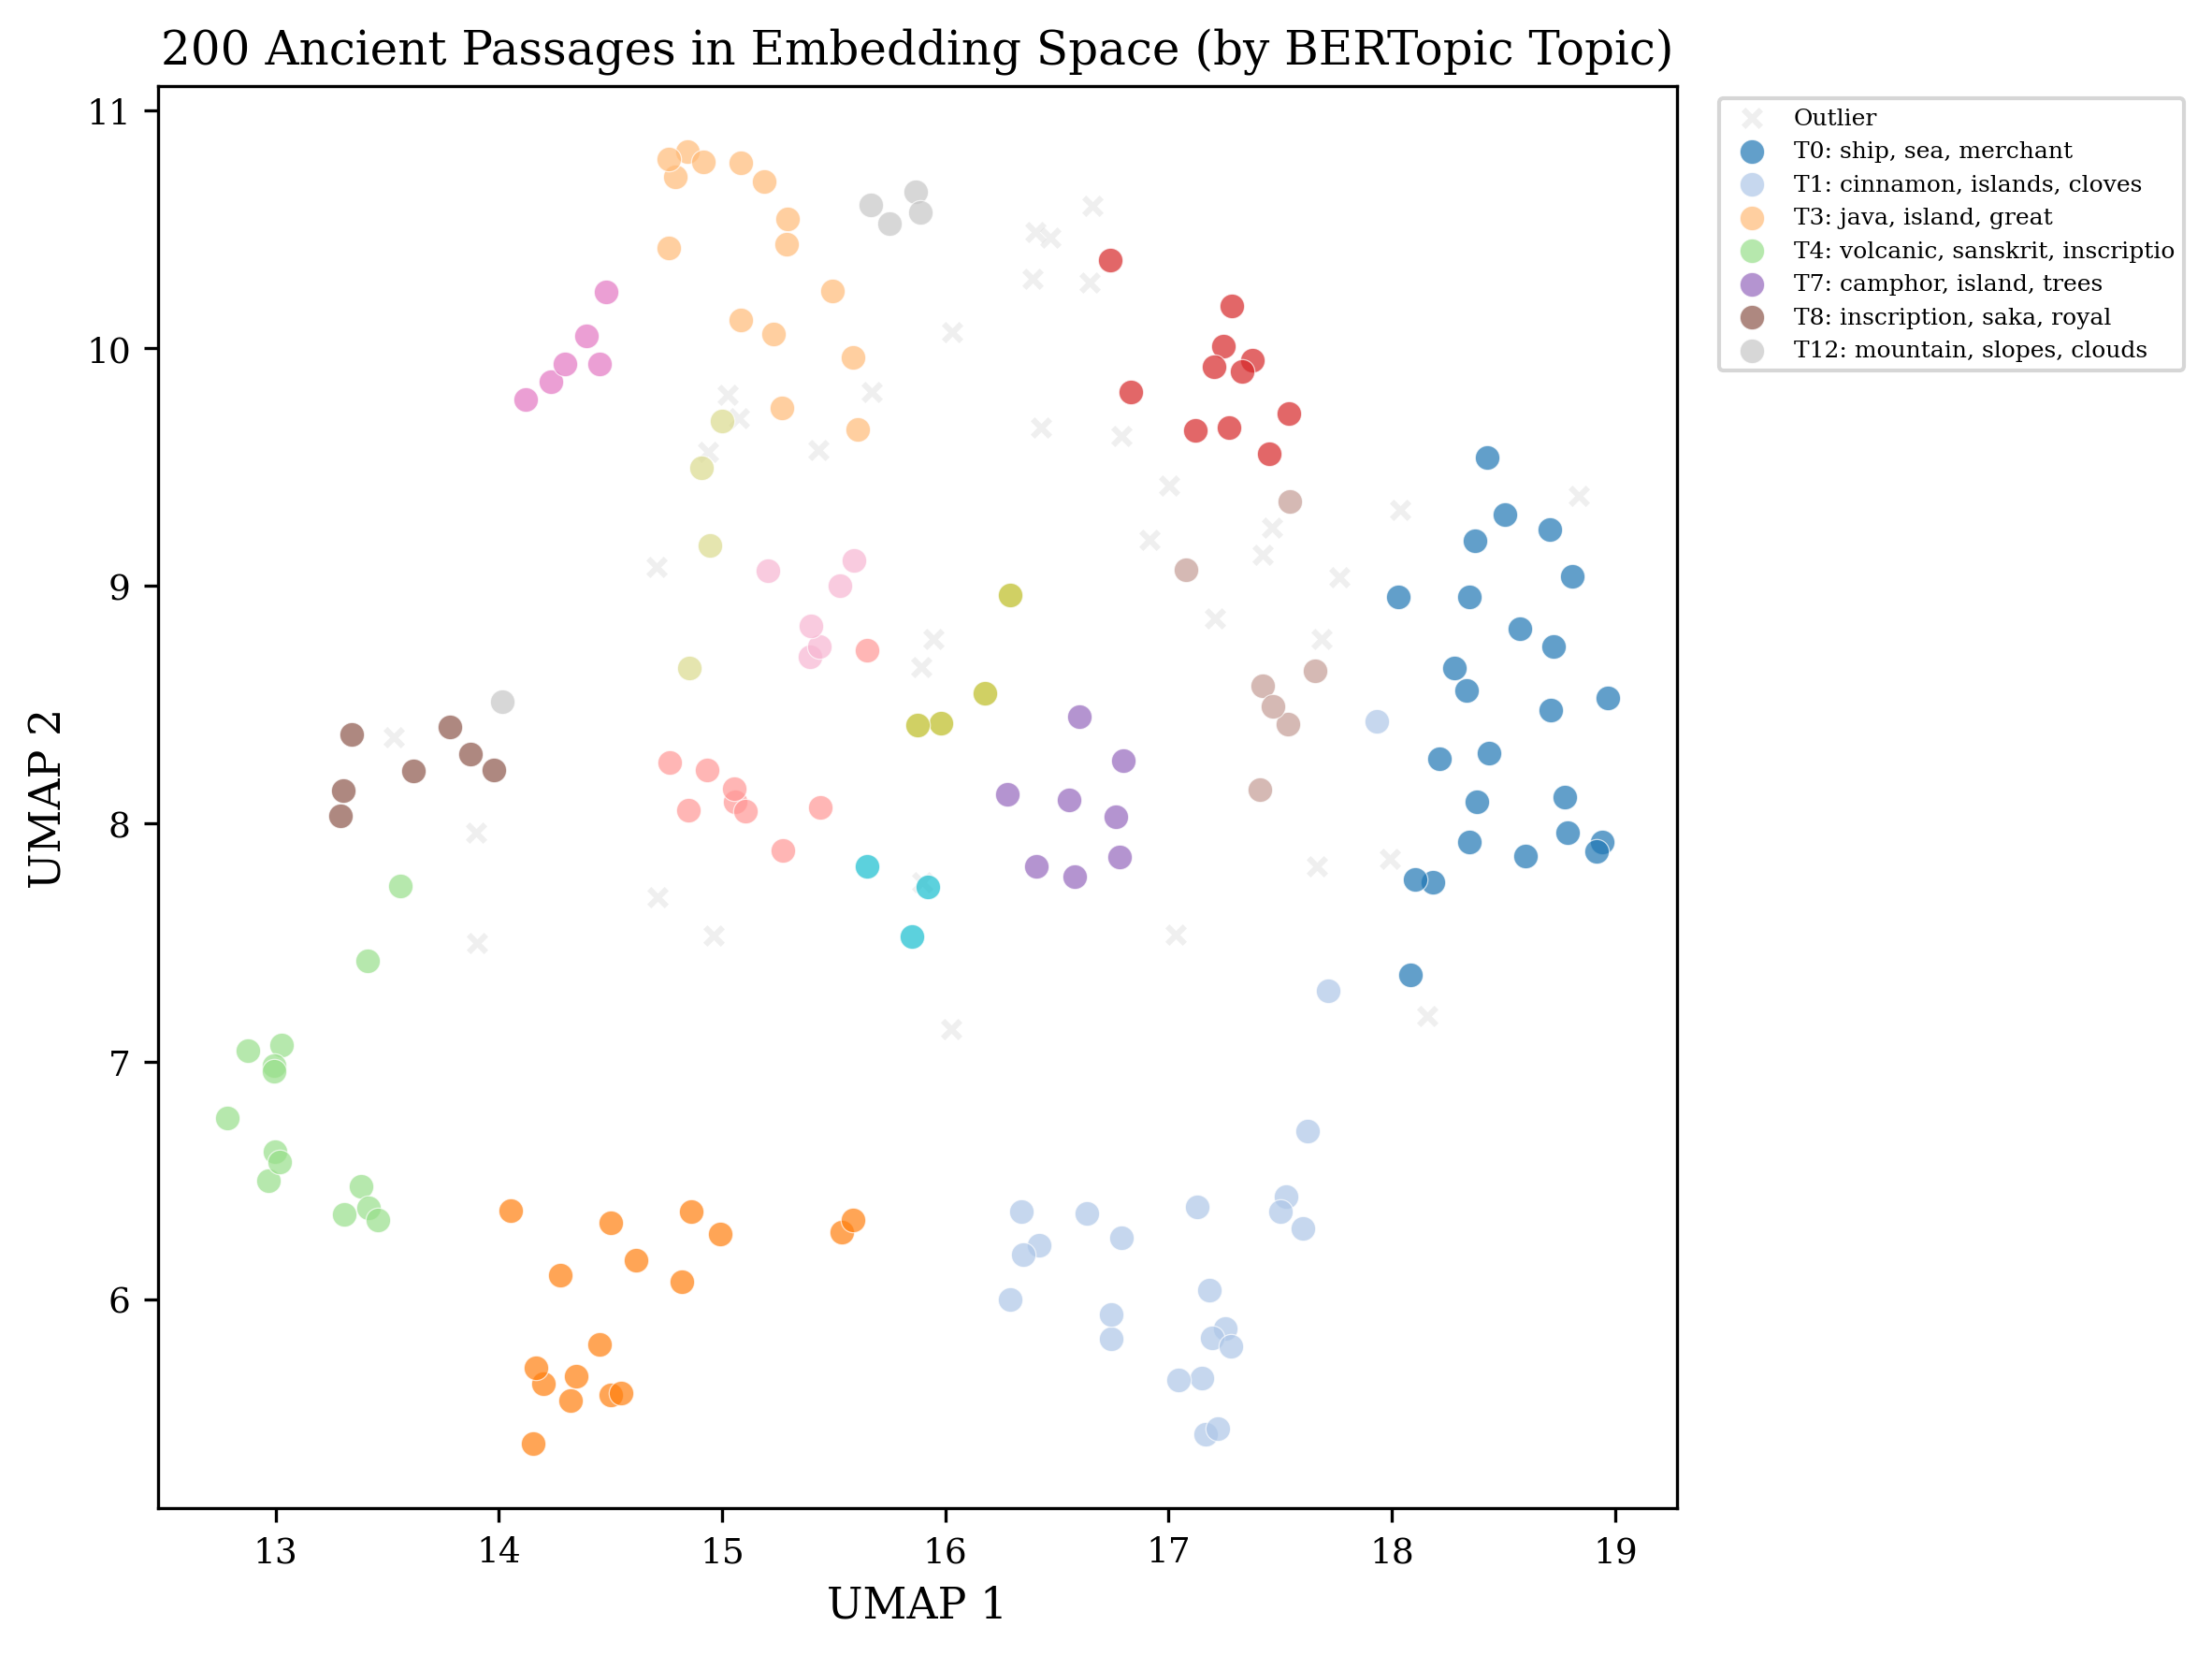
\includegraphics[width=0.48\textwidth]{figures/fig2_umap_topic.png}
\caption{UMAP projection of 200 ancient passages encoded with Sentence-BERT. \textbf{Left:} Colored by tradition of origin---traditions mix spatially, confirming content-driven clustering. \textbf{Right:} Colored by BERTopic topic---16 latent topics emerge, including Topic~4 (volcanic/inscriptions) and Topic~12 (mountain/landscape).}
\label{fig:umap}
\end{figure}

\subsection{Volcanic silence in epigraphy}

The seven semantic queries against the DHARMA corpus yield a striking pattern (Figure~\ref{fig:queries}).
``Mountain worship and sacred peaks'' achieves the \emph{highest} mean similarity to inscriptional content ($\bar{s} = 0.395$), while ``volcanic landscape fire mountain'' achieves the \emph{lowest} ($\bar{s} = 0.244$).
The gap of $0.151$ in cosine similarity is substantial in the context of SBERT embeddings, where typical within-tradition vs.\ between-tradition differences are on the order of $0.09$ (Section~4.1 of the cross-tradition analysis).

This means that mountains appear abundantly in inscriptions---but as sacred, cosmological sites, not as geological or volcanic features.
The Kakawin Ramayana describes Penanggungan as a cosmic mountain; no inscription describes Merapi as a destructive volcano, despite its eruptions burying nearby temples at depths of 5--7 metres \citep{Newhall2000}.
The inscriptional genre encodes the \emph{cosmological} mountain while excluding the \emph{physical} mountain.

\begin{figure}[htbp]
\centering
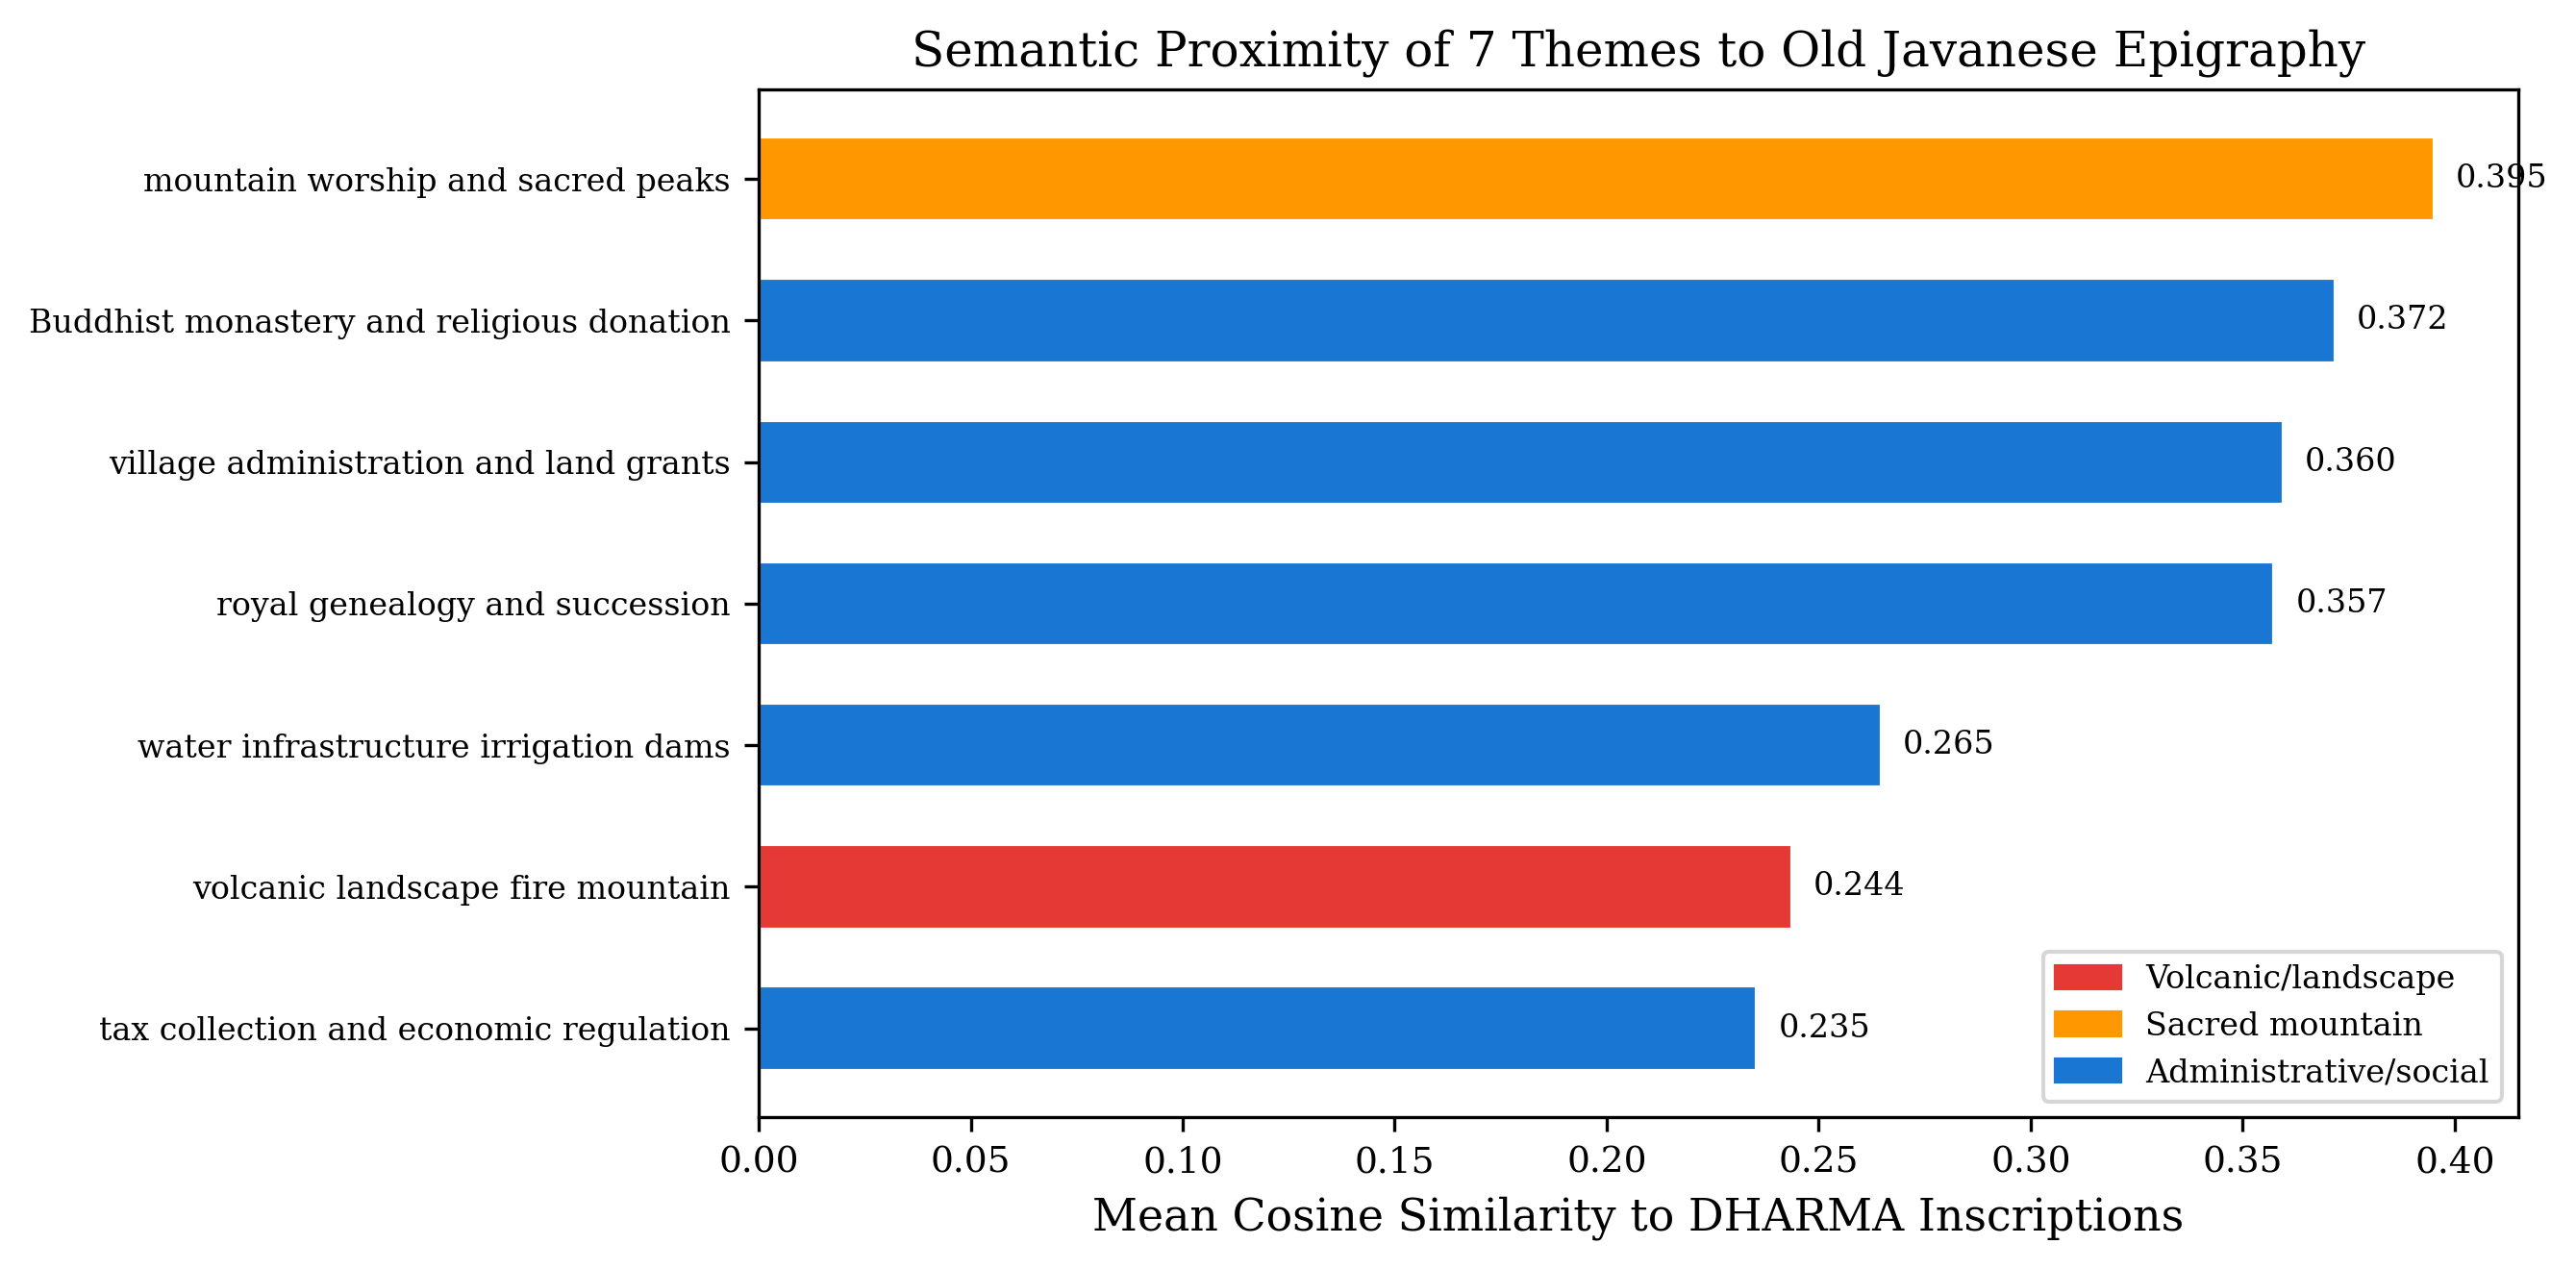
\includegraphics[width=\textwidth]{figures/fig4_query_similarities.png}
\caption{Mean cosine similarity between seven thematic queries and 173 DHARMA inscription embeddings. ``Volcanic landscape fire mountain'' (red) achieves the \emph{lowest} similarity, while ``mountain worship and sacred peaks'' (orange) achieves the \emph{highest}---a gap of 0.151 in cosine similarity.}
\label{fig:queries}
\end{figure}

\subsection{The 929 CE discursive discontinuity}

BERTopic applied to 46 dated inscriptions yields three topics: \textbf{T0} (administrative, 28 documents), \textbf{T1} (royal/political, 10 documents), and \textbf{T2} (ritual/calendrical, 6 documents).

Across the 929 CE divide the topic distribution shifts (Fisher's exact $p = 0.0003$; a $\chi^2$ is unreliable here because several expected cell counts fall below five). With only 33 pre-929 and 13 post-929 inscriptions, we read this as suggestive rather than definitive (Figure~\ref{fig:heatmap}).
Before 929 CE, administrative discourse dominates (70\%, 23/33) with ritual/calendrical formulas as secondary (18\%, 6/33).
After 929 CE, royal/political discourse surges to 62\% (8/13), administrative declines to 38\% (5/13), and ritual/calendrical discourse is absent in this subset (0/13, down from 6/33 pre-929).

A Fisher's exact test indicates an increase in Topic~1 (royal/political) discourse ($\text{OR} \approx 25$, $p = 0.0002$), though this rests on small subsamples (4 vs.\ 8 inscriptions) and should be read as indicative rather than precise.

\begin{figure}[htbp]
\centering
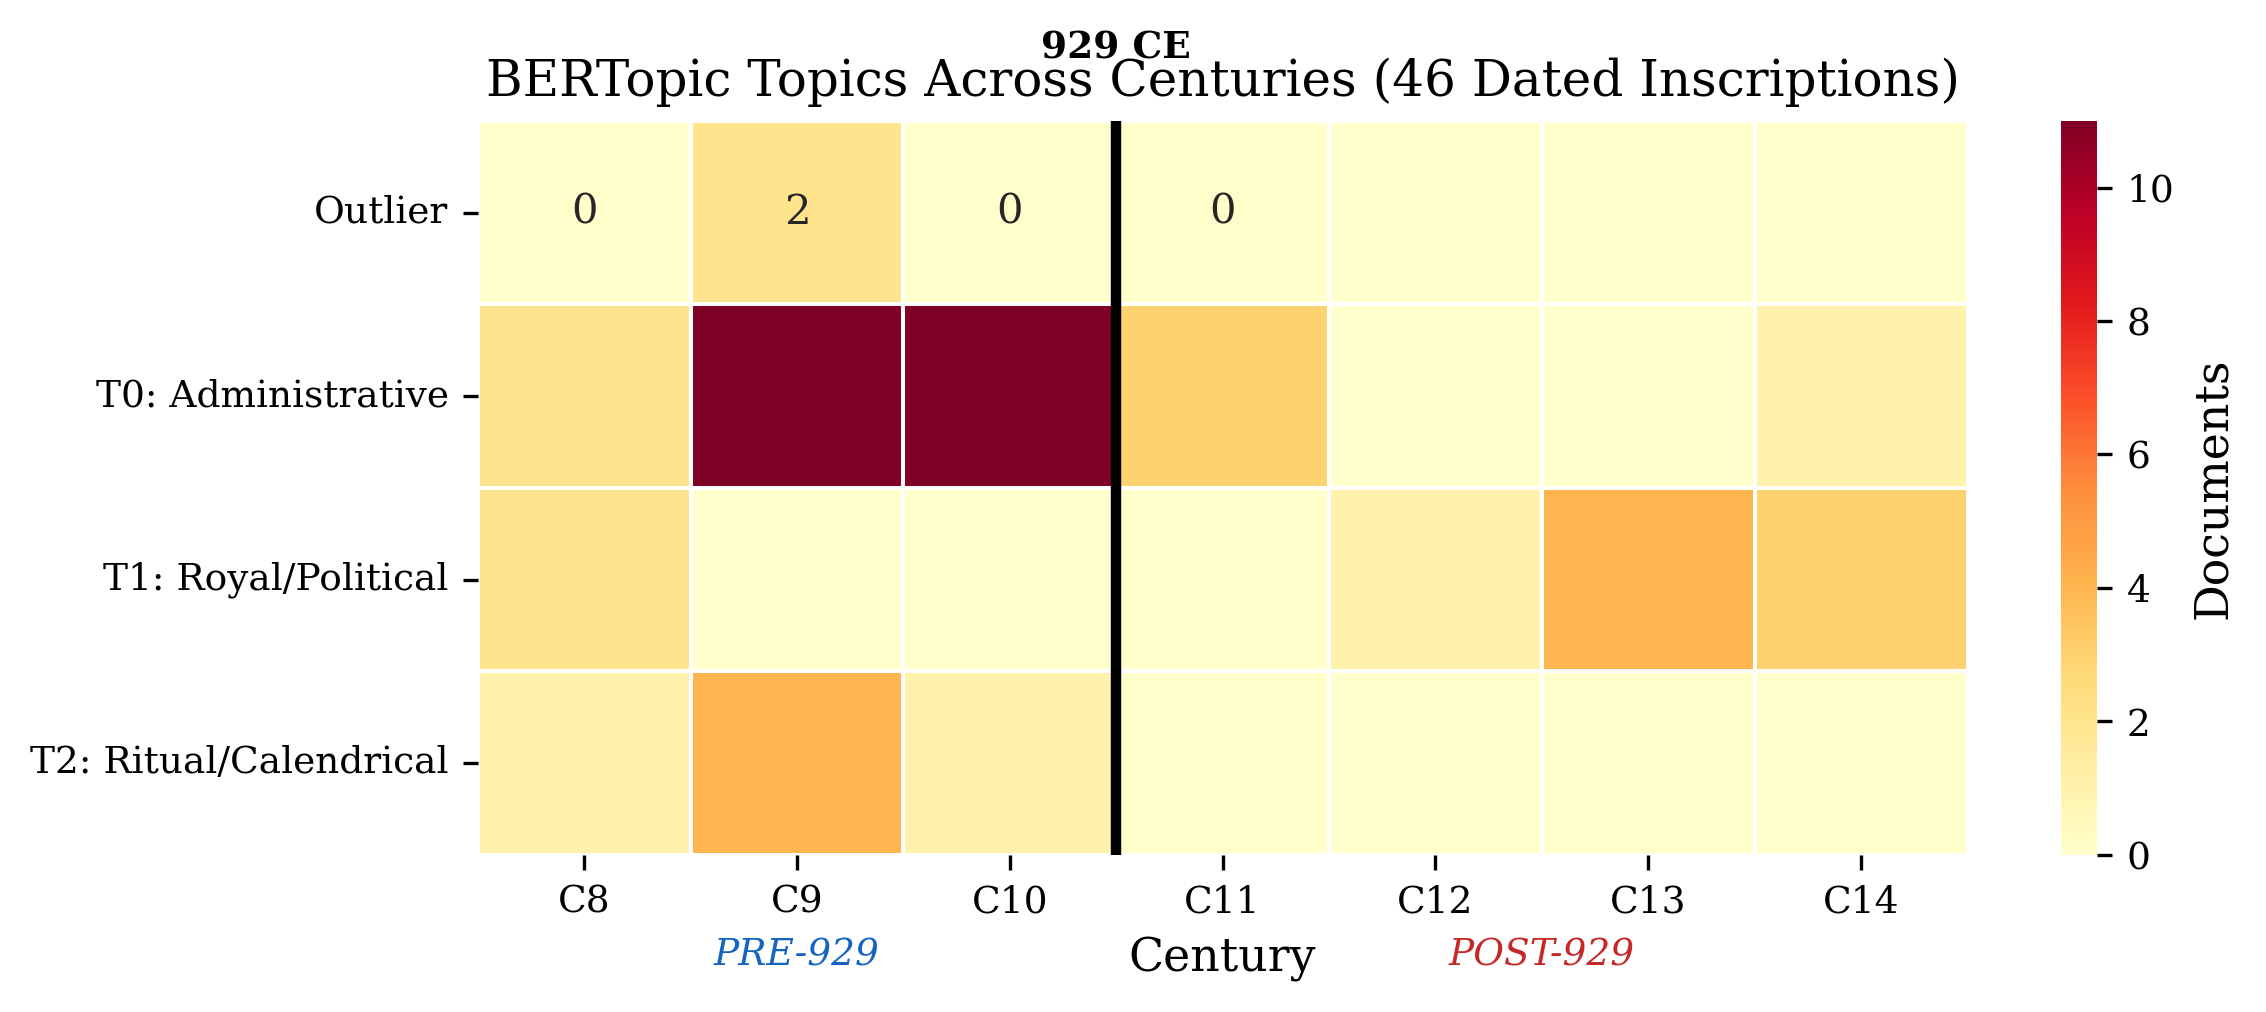
\includegraphics[width=\textwidth]{figures/fig5_topic_heatmap.png}
\caption{BERTopic topic distribution across centuries for 46 dated DHARMA inscriptions. The vertical black line marks the 929 CE Mataram collapse. Administrative discourse (T0) dominates pre-929; royal/political discourse (T1) dominates post-929. Ritual/calendrical formulas (T2) are absent in the post-929 subset (based on only 6 pre-929 instances).}
\label{fig:heatmap}
\end{figure}

Temporal centroid drift analysis (Figure~\ref{fig:drift}) shows that the largest semantic rupture occurs not at the 929 CE divide (C10$\rightarrow$C11 distance $= 0.208$) but at the C11$\rightarrow$C12 transition ($0.366$).
Because the discursive change is therefore \emph{not} tightly aligned in time with the political collapse, we treat the association with 929 CE cautiously: the transformation appears gradual (consistent with institutional inertia) rather than a sharp response to the 929 CE event.

\begin{figure}[htbp]
\centering
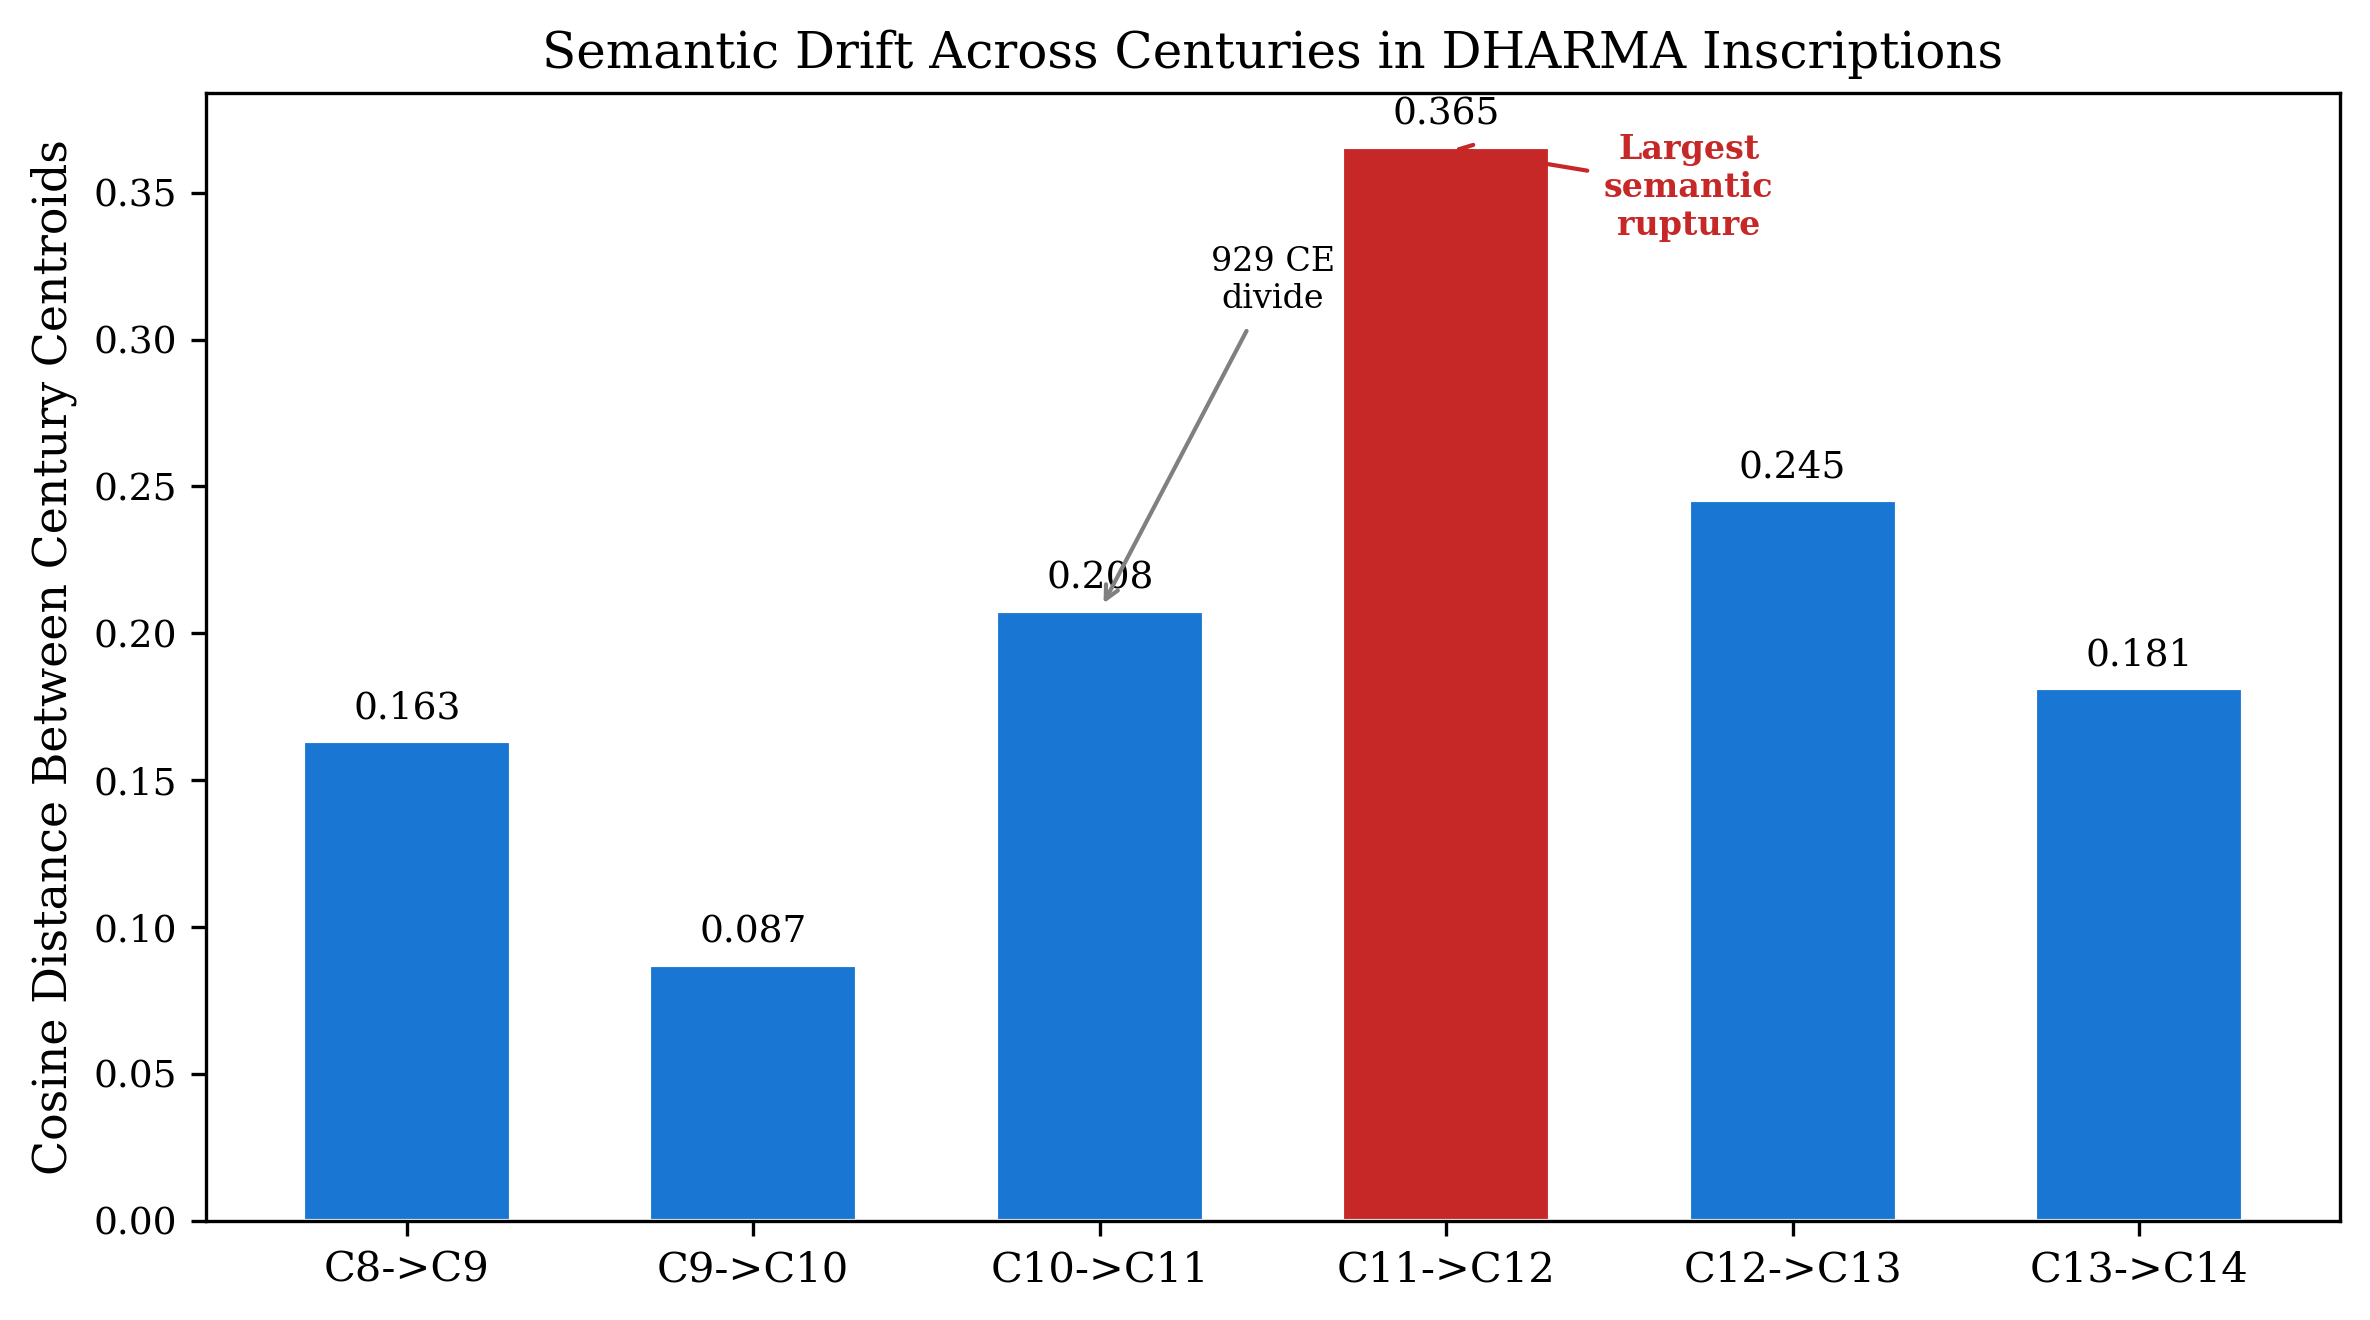
\includegraphics[width=\textwidth]{figures/fig6_temporal_drift.png}
\caption{Cosine distance between consecutive century centroids in DHARMA inscription embedding space. The C11$\rightarrow$C12 transition (red) shows the largest semantic rupture, exceeding the 929 CE divide (C10$\rightarrow$C11).}
\label{fig:drift}
\end{figure}

\subsection{Cross-lingual validation}

The cross-lingual analysis yields one honest negative and one informative positive result.

\textbf{XLM-RoBERTa-base} produces near-uniform embeddings via mean pooling (mean pairwise similarity $= 0.997$), effectively collapsing all inscriptions to a single point in embedding space.
This is a known limitation of token-level models applied to sentence-level similarity tasks without fine-tuning: XLM-R was not trained for sentence comparison and its mean-pooled representations lack discriminative power.
Despite this, the relative ordering of thematic queries is partially preserved: ``volcanic landscape'' still scores lowest even in the compressed space ($0.9868$), and the Spearman correlation with SBERT rankings is significant ($\rho = 0.452$, $p < 10^{-300}$).

\textbf{Multilingual SBERT} produces informative results (Table~\ref{tab:crosslingual}).
The correlation between original-language and English-translation similarity structures is significant and positive ($\rho = 0.336$, $p < 10^{-164}$), confirming that the English-only analysis captures real semantic structure.
However, the moderate correlation indicates that translation mediates similarity in ways that both introduce and remove information.

\begin{table}[htbp]
\centering
\caption{Cross-lingual semantic query comparison: Multilingual SBERT on original Old Javanese vs English SBERT on translations.}
\label{tab:crosslingual}
\begin{tabular}{lrrrr}
\toprule
\textbf{Query} & \textbf{ML-SBERT} & \textbf{EN-SBERT} & \textbf{Rank (OJ)} & \textbf{Rank (EN)} \\
\midrule
Buddhist monastery       & 0.330 & 0.372 & 1 & 2 \\
Mountain worship         & 0.253 & 0.395 & 2 & 1 \\
Village administration   & 0.167 & 0.360 & 3 & 3 \\
Volcanic landscape       & 0.156 & 0.244 & 4 & 6 \\
Royal genealogy          & 0.114 & 0.357 & 5 & 4 \\
Water infrastructure     & 0.092 & 0.265 & 6 & 5 \\
Tax/economic regulation  & 0.012 & 0.235 & 7 & 7 \\
\bottomrule
\end{tabular}
\end{table}

Three findings emerge from the cross-lingual comparison.
First, \emph{volcanic themes score in the lower half in both analyses}---rank 4 of 7 in original Old Javanese and rank 6 of 7 in English. The effect is weaker in the original language: volcanic discourse is intermediate (rank 4/7), not lowest, so the pronounced ``silence'' seen in English is partly translation-dependent. The consistent below-average ranking in both languages indicates the under-representation is not \emph{solely} a translation artefact, even if its magnitude is.
Second, Buddhist content rises to the highest rank in original-language analysis ($0.330$), because the Sanskrit and Pali vocabulary in inscriptions is directly captured by the multilingual model, whereas English translation flattens liturgical vocabulary.
Third, tax and economic regulation collapses to near-zero similarity in original-language analysis ($0.012$), because the English administrative terms (``tax,'' ``regulation,'' ``economic'') have no direct cross-lingual equivalents in Old Javanese word forms---the translation introduces semantic similarity that does not exist in the original.

These results validate the English-only analysis as a legitimate first-order approximation while revealing that translation both enhances and distorts thematic similarity.
For volcanic themes specifically, the cross-lingual validation \emph{tempers} the strong English result: volcanic discourse ranks below average in both languages (direction robust), but the pronounced ``silence'' (lowest of seven) holds only in English, not in the original Old Javanese (rank 4 of 7). We therefore frame this as a relative under-representation of volcanic-geological themes in inscriptions---robust in direction, modest in magnitude.


\section{Discussion}

\subsection{Computational evidence for textual taphonomic bias}

Our three analyses are consistent with a single interpretation: the Indonesian textual record is shaped by genre-specific selection pressures that under-represent certain categories of information.

External traditions describe a Nusantara rich in volcanic landscapes, geological features, and material commodities.
The \textsc{volcano} concept converges across all 12 traditions ($z_\mathrm{cross} = 7.1$), and BERTopic discovers a latent ``volcanic landscape'' topic (Topic~12) comprising passages from multiple traditions.
Yet when we query the DHARMA inscriptional corpus for volcanic or landscape themes, we obtain the lowest similarity of any tested theme ($0.244$).

This is not because ancient Javanese were unaware of volcanism---the cross-tradition evidence, combined with the physical evidence of temples built on volcanic slopes \citep[submitted]{Amien2026b}, demonstrates awareness.
Rather, the inscriptional genre served administrative and legitimatory purposes: inscriptions record land grants, tax exemptions, royal genealogies, and religious endowments, and largely do not describe physical geography.
The pattern---abundant cosmological mountains, scarce geological ones---is consistent with genre-specific selection rather than ignorance.
We cannot fully exclude alternatives: volcanic phenomena may be encoded in Old Javanese vocabulary (e.g.\ \emph{gunung}, eruption verbs) not captured by an English query, and some cross-tradition agreement may reflect shared reliance on Indian or Chinese intermediary sources. But the convergence-versus-exclusion contrast, robust in direction across languages, is most parsimoniously read as genre-driven selection.

\subsection{The 929 CE shift as discursive transformation}

The statistically significant topic redistribution at 929 CE reveals that political collapse does not merely change \emph{where} inscriptions are written---it changes \emph{what they say}.
The disappearance of ritual/calendrical formulas (Topic~2) and the surge of royal legitimation language (Topic~1) suggest that the post-929 East Javanese kingdoms used inscriptions primarily for political purposes, abandoning the administrative and ritual functions that characterized Central Javanese epigraphy.

This has implications for archaeological interpretation.
If we use inscriptions as proxies for settlement density or economic activity, the pre-929/post-929 comparison is not like-for-like.
The genres are different, the information encoded is different, and any inference drawn from inscription counts alone conflates taphonomic bias with historical signal.

\subsection{Methodological contribution: computational textual archaeology}

This paper demonstrates that transformer-based NLP can extract meaningful structure from ancient and translated corpora, even when the texts span radically different languages, periods, and genres.
We propose the term \emph{computational textual archaeology} for this approach: the use of computational methods to recover information about past societies from the structure of their textual record, treating text not merely as a source of facts but as an artefact shaped by the same taphonomic processes that shape material remains.

The specific pipeline---SBERT encoding, Monte Carlo convergence testing, BERTopic topic discovery, and semantic query analysis---is fully reproducible and requires no task-specific training data.
The only input is translated text; the output is a quantitative characterization of what a corpus encodes and, by comparison with external evidence, what it excludes.
This makes the pipeline directly transferable to other ``archaeological darkness'' problems.
Sub-Saharan African history, where external Arabic and Portuguese sources describe complex polities that left limited indigenous inscriptions, is an obvious candidate.
Pre-colonial Pacific archaeology, where oral traditions and European contact narratives exist alongside sparse material records, is another.
In each case, the question is the same: does external textual evidence converge on themes that indigenous records exclude?

The DHARMA EpiDoc corpus, in TEI-XML format, proved well-suited for computational analysis.
The structured markup enabled automated extraction of translations, dates, languages, and find-spot metadata without manual preprocessing.
As more epigraphic corpora are digitized in structured formats---a trend accelerated by projects like DHARMA, EAGLE, and I.Sicily---the methods presented here can be applied at scale.

\subsection{The recursive nature of textual bias}

Our findings suggest a recursive relationship between taphonomic bias at different levels.
Physical burial (volcanic sedimentation) removes material evidence from Volcano Java.
Survey deficit (institutional under-investment) fails to recover what burial conceals.
And textual genre taphonomy (inscriptional exclusion of physical geography) ensures that even the surviving textual record does not describe what is being buried.

These three biases compound one another.
Inscriptions were produced by and for court centres, and their surviving content is thematically biased toward administrative and legitimatory functions rather than the physical landscape.
A researcher relying solely on inscriptions would therefore reconstruct ancient Java as a world of royal courts, land grants, and Buddhist endowments---with little trace of the parallel world of sacred architecture and indigenous practice on the volcanic slopes.

This recursion is not unique to Indonesia.
Any region where textual production was institutionally concentrated---and where natural processes differentially preserve or destroy evidence from different zones---is likely to exhibit similar compound bias.
The contribution of computational textual archaeology is to make this bias measurable.

\subsection{Limitations}

Several limitations should be acknowledged.
First, the primary analyses use English translations rather than original-language texts.
Our cross-lingual validation (Section~5.5) demonstrates that the major patterns---particularly volcanic silence---are robust across languages, but the moderate correlation ($\rho = 0.336$) between original and translated similarity structures indicates that translation mediates semantic relationships in non-trivial ways.
Fine-tuned multilingual models for Old Javanese would provide a stronger test, but no such models currently exist.

Second, the diachronic analysis is constrained by the small number of dated inscriptions with translations ($n = 46$), which limits statistical power for individual topic comparisons.
The overall chi-square test ($p = 0.0003$) and the Fisher's exact test for Topic~1 ($p = 0.0002$) are highly significant, but the disappearance of Topic~2 (ritual/calendrical formulas) post-929 involves only 6 pre-929 instances and cannot be tested independently.

Third, SBERT (all-MiniLM-L6-v2) is trained on modern English and may miss semantic nuances specific to ancient translated texts.
The translations themselves vary in style and date of composition, introducing an additional layer of semantic mediation.

Fourth, corpus construction involved subjective decisions about passage selection and thematic tagging.
The Monte Carlo convergence test is designed to be robust to moderate tagging errors (a concept group need only contain a majority of relevant passages, not be perfectly curated), but the choice of which concept groups to test introduces researcher degrees of freedom.
We mitigate this by reporting all eight groups tested, including the weakest result (\textsc{metal\_trade}, $z = 2.71$).

Fifth, the cross-lingual validation reveals that XLM-RoBERTa-base is unsuitable for this task without fine-tuning---a limitation of current multilingual transformers for low-resource ancient languages.
Future work should explore domain-adapted models or fine-tuning on aligned ancient-modern text pairs.


\section{Conclusion}

Three independently derived computational findings converge on the same conclusion.
Ancient textual traditions converge on Nusantaran themes \emph{across traditions} ($8/8$ concept groups, strongest $z_\mathrm{cross} = 32.2$), inscriptions under-represent physical geography (volcanic-geological themes rank below average---lowest in English, rank 4/7 in original Old Javanese), and a sample-limited discursive shift accompanies the 929 CE Mataram transition (Fisher's exact $p = 0.0003$, $n = 46$).

Together, these findings are consistent with a form of taphonomic bias that operates not in the soil but in the stone---not through volcanic burial but through genre selection.
The archaeological darkness of Indonesia may be shaped not only by what the earth conceals but by what inscriptions choose not to record.
The cross-lingual validation indicates this is not \emph{solely} a translation artefact: volcanic-geological themes rank below average in both languages ($\rho = 0.336$ between original and translated similarity structures), though the effect is weaker in the original Old Javanese (rank 4/7).

Understanding this bias is essential for any attempt to use textual evidence as a proxy for past human activity in volcanically active regions.
The implications extend beyond Indonesia: wherever inscriptional corpora are used to reconstruct past societies, the genre-specific selection pressures that determined what was inscribed---and what was not---must be accounted for.
The gap between what external sources report and what internal records encode is not noise; it is a measurable signal of textual taphonomy.

The methods presented here---semantic convergence testing, latent topic discovery, epigraphic semantic search, and cross-lingual validation---constitute a toolkit for ``computational textual archaeology'' that can be applied wherever the gap between external references and internal records raises questions about what the past chose to remember and what it chose to forget.


\subsection*{Data availability}

The cross-tradition corpus (E089 v5) and all analysis scripts are available in the VOLCARCH repository: \url{https://github.com/mukhlisamien/volcarch}.
The DHARMA inscriptions are available from the DHARMA project: \url{https://github.com/erc-dharma}.
To support full reproducibility, the corpus-construction protocol---the passage-selection criterion, the thematic tagging rubric for the eight concept groups, and the seven epigraphic query definitions---is documented alongside the embedding and analysis code in the repository.

\subsection*{AI Disclosure}

This research employed an AI-augmented workflow using Claude (Anthropic) for
literature synthesis, NLP pipeline development (SBERT encoding, UMAP clustering,
BERTopic, Monte Carlo convergence testing), cross-corpus comparison, and
manuscript drafting assistance.
The research hypotheses, domain interpretation, ethical decisions, and final
scholarly judgments were made by the human author.
All AI-generated code, statistical results, and manuscript text were reviewed,
validated, and edited by the author.


\subsection*{Acknowledgements}

The author thanks the DHARMA project (ERC Synergy Grant No.\ 809994) for making the EpiDoc inscription corpus publicly available, and the ABVD, GVP, and Smithsonian Institution for open archaeological and volcanological datasets.

\subsection*{About the author}
Mukhlis Amien is a lecturer at the Lab Data Sains, Universitas Bhinneka Nusantara, Malang. His research interests are computational linguistics and natural language processing, digital humanities, computational epigraphy, and the archaeology and historical linguistics of insular Southeast Asia. His recent work includes a preprint on the computational detection of phonological substrates in Austronesian languages (arXiv:2604.00023). He can be reached at amien@ubhinus.ac.id.

\bibliography{p16_references}

\end{document}
